% !TEX root = learner4_slides.tex
% Short slide deck: Learner 4 / order-reduction simulation (H0 preliminary evidence).
% Build: pdflatex -output-directory=../outputs/learner4 learner4_slides.tex
%    or: ./scripts/build_learner4_slides.sh
\documentclass[aspectratio=169, 11pt]{beamer}

\usetheme{Madrid}
\usecolortheme{whale}
\setbeamertemplate{navigation symbols}{}
\setbeamertemplate{footline}[frame number]
\setbeamertemplate{blocks}[rounded][shadow=false]

\usepackage{amsmath,amssymb}
\usepackage{graphicx}
\usepackage{booktabs}
\usepackage{xcolor}

\definecolor{passgreen}{HTML}{1E8449}
\definecolor{failred}{HTML}{C0392B}
\definecolor{accentblue}{HTML}{2471A3}

\title[Learner 4: order reduction]{Do we co-contract in order to learn?}
\subtitle{Preliminary simulation evidence for H0 (URF proposal \emph{Tuning to Learn})}
\author{Dipankar Bhattacharya}
\date{\today}

\begin{document}

% =========================================================================
\begin{frame}
\titlepage
\end{frame}

% =========================================================================
\begin{frame}{Basic idea}
\begin{columns}[T]
\begin{column}{0.52\linewidth}
\begin{block}{The claim (H0)}
A complicated object is made \textbf{learnable} by tuning your own body to
\textbf{simplify} it --- not only to stabilise it.
\end{block}
\vspace{4pt}
\begin{itemize}
  \item Carry a cup of coffee: a \textbf{slow} displacement (dominant
        dynamics) plus a \textbf{fast} wobble (transients).
  \item Co-contraction (bracing) pushes the fast poles deeper into the
        left half-plane.
  \item The fast wobble settles \emph{within the movement} $\Rightarrow$
        it becomes filtered noise.
  \item What is left to learn is only the dominant, slow dynamics.
\end{itemize}
\end{column}
\begin{column}{0.44\linewidth}
\centering
\begin{block}{Question tested here}
\centering
\emph{Does bracing actually make the dominant dynamics faster and safer
to learn --- and can you still recover the rest later?}
\end{block}
\end{column}
\end{columns}
\end{frame}

% =========================================================================
\begin{frame}{Overall block diagram}
\centering
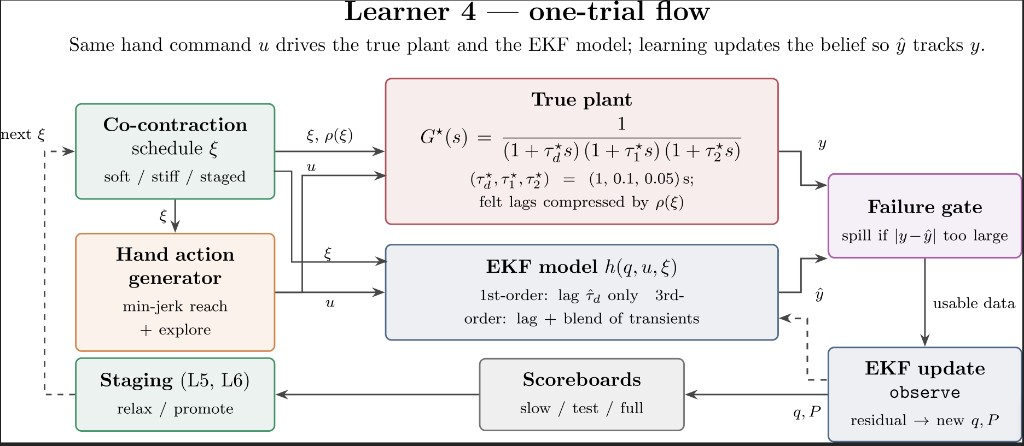
\includegraphics[width=0.92\linewidth]{../outputs/learner4/learner4_block_diagram_modified.png}
\end{frame}

% =========================================================================
\begin{frame}{What is a trial? What is a seed?}
\begin{columns}[T]
\begin{column}{0.48\linewidth}
\begin{block}{One trial}
One out-and-back reach with the cup.
\vspace{4pt}
\begin{itemize}
  \item Duration $T=2.5$\,s, sample $\Delta t=0.01$\,s
        ($n_t=250$ samples).
  \item Movement time fixed: $t_{\mathrm{move}}=0.25$\,s.
  \item Pick grip $\xi$, generate hand path $u$,
        feel $y$, predict $\hat y$, maybe update belief.
  \item Can \textbf{fail} (``spill'') if
        $|y-\hat y|$ exceeds tolerance --- then learning
        uses only the usable prefix, or none.
\end{itemize}
\vspace{4pt}
{\footnotesize Figures report medians over \textbf{60 trials}
per seed.}
\end{block}
\end{column}
\begin{column}{0.48\linewidth}
\begin{block}{One seed}
One independent run of the whole experiment
(a fresh random generator).
\vspace{4pt}
\begin{itemize}
  \item Exploration noise and sensor noise differ
        across seeds.
  \item Same strategy, same plant, different
        random realisations.
  \item We run \textbf{20 seeds} and report
        medians / means so one lucky noise draw
        cannot decide the story.
\end{itemize}
\vspace{4pt}
{\footnotesize Think: 20 simulated people, each doing
60 reaches under one strategy.}
\end{block}
\end{column}
\end{columns}
\end{frame}

% =========================================================================
\begin{frame}{Block diagram --- notation and formulas}
\small
\begin{center}
\begin{tabular}{@{}ll@{}}
\toprule
\textbf{Symbol} & \textbf{Meaning / formula} \\
\midrule
$\xi$
  & Co-contraction (grip). Soft $\xi\approx0.7$; stiff $\xi\approx3$. \\
$\rho(\xi)$
  & Separation ratio:
    $\rho=(\xi+\sqrt{\xi^2-1})^2$ if $\xi>1$, else $1$. \\
$u$
  & Hand command:
    $u=u_{\mathrm{ref}}+0.10\,u_{\mathrm{explore}}$
    (min-jerk + band-limited noise). \\
$G^\star(s)$
  & True plant:
    $\displaystyle\frac{1}{(1+\tau_d^\star s)(1+\tau_1^\star s)(1+\tau_2^\star s)}$,
    $\tau^\star=(1,\,0.1,\,0.05)$\,s. \\
Felt lags
  & $(\tau_d^\star,\;\tau_1^\star/\rho,\;\tau_2^\star/\rho)$
    --- only fast poles compressed. \\
$y$
  & Measurement: cascade of felt lags on $u$, plus noise
    ($0.012\,\varepsilon$). \\
$q,\,P$
  & EKF belief and covariance
    (1st-order: $\log\hat\tau_d$;
     3rd: also $\log\hat\tau_{1,2},\,w_{1,2}$). \\
$h(q,u,\xi)$
  & Measurement model $\to$ prediction $\hat y$. \\
$n_{\mathrm{eff}}$
  & Effective order $=1+w_1+w_2$ (how many modes are ``on''). \\
Failure
  & Spill if $|y[k]-\hat y[k]|>0.15\cdot\xi/\xi_{\mathrm{soft}}$. \\
\bottomrule
\end{tabular}
\end{center}
\end{frame}

% =========================================================================
\begin{frame}{One-trial flow (through the diagram)}
\small
\begin{enumerate}
  \item[\textbf{1.}] \textbf{Schedule} picks $\xi$ for this trial
        (soft / stiff / staged).
  \item[\textbf{2.}] \textbf{Hand action generator} builds
        $u$ (same out-and-back path + small wiggles).
  \item[\textbf{3.}] \textbf{True plant} gets $(u,\xi)$:
        compresses fast lags by $\rho(\xi)$, cascades them,
        adds noise $\to$ felt $y$.
  \item[\textbf{4.}] \textbf{EKF model} gets the \emph{same} $(u,\xi)$
        and current belief $q$ $\to$ predicted feel $\hat y=h(q,u,\xi)$.
  \item[\textbf{5.}] \textbf{Failure gate} compares $y$ and $\hat y$.
        If mismatch is too large, truncate (spill); else keep the trial.
  \item[\textbf{6.}] \textbf{EKF update} (\texttt{observe}): residual
        $y-\hat y$ nudges $q$ and shrinks $P$
        (or \texttt{drift} if too little usable data).
  \item[\textbf{7.}] \textbf{Scoreboards} log slow / soft-probe / full-object error
        [how well we know the slow lag; whether we could carry the cup softly
        now; and how good our full model of the cup is].
  \item[\textbf{8.}] \textbf{S3 (brace then hand over)}: if confident enough,
        relax $\xi$ and hand the slow estimate to a fuller soft model
        (S2 stays braced forever and never does this step).
\end{enumerate}
\vspace{4pt}
\begin{block}{Key point}
Same $u$ drives world and brain. Learning is nothing more than updating $q$
so that $\hat y$ tracks $y$.
\end{block}
\end{frame}

% =========================================================================
\begin{frame}{The object and the learner}
\begin{columns}[T]
\begin{column}{0.5\linewidth}
\textbf{True plant} (never changes):
\[
G(s)=\frac{1}{(1+\tau_d s)(1+\tau_1 s)(1+\tau_2 s)}
\]
\[
(\tau_d,\tau_1,\tau_2) = (1.0,\,0.1,\,0.05)\ \mathrm{s}
\]
One slow pole (dominant dynamics), two fast poles (wobbles).
\vspace{6pt}

Co-contraction $\xi$ compresses the fast poles by
\[
\rho(\xi) = \bigl(\xi+\sqrt{\xi^2-1}\bigr)^2,\quad \xi>1.
\]
\end{column}
\begin{column}{0.5\linewidth}
\textbf{The learner}: an extended Kalman filter (EKF)
\begin{itemize}
  \item Carries a belief over the time constants.
  \item Predicts the felt force from hand motion $+$ grip.
  \item Updates from the residual (predicted vs.\ felt).
  \item Unused fast modes are pruned toward ``off''
        (automatic relevance prior).
  \item Effective model order $n_{\mathrm{eff}}$ reads off how many
        modes currently participate.
\end{itemize}
\end{column}
\end{columns}
\end{frame}

% =========================================================================
\begin{frame}{How $G(s)$ is scaled by $\rho(\xi)$}
\small
\textbf{Object itself never changes:}
\[
G^\star(s)=\frac{1}{(1+\tau_d^\star s)\,(1+\tau_1^\star s)\,(1+\tau_2^\star s)},
\qquad (\tau_d^\star,\tau_1^\star,\tau_2^\star)=(1.0,\,0.1,\,0.05)\,\mathrm{s}.
\]
\vspace{2pt}
\textbf{What co-contraction changes} is the \emph{felt} plant: only the fast lags are divided by $\rho(\xi)$:
\[
\rho(\xi)=\begin{cases}
1 & \xi\le 1,\\[2pt]
\bigl(\xi+\sqrt{\xi^{2}-1}\bigr)^{2} & \xi>1,
\end{cases}
\qquad
G_{\mathrm{felt}}(s)=\frac{1}{(1+\tau_d^\star s)\,(1+\tfrac{\tau_1^\star}{\rho}s)\,(1+\tfrac{\tau_2^\star}{\rho}s)}.
\]
\vspace{4pt}
\begin{center}
\begin{tabular}{@{}cccc@{}}
\toprule
Grip & $\xi$ & $\rho(\xi)$ & Felt lags $(\tau_d,\,\tau_1/\rho,\,\tau_2/\rho)$ \\
\midrule
Soft  & $0.7$ & $1$ & $(1.0,\;0.10,\;0.05)$\,s --- all three visible \\
Stiff & $3.0$ & $\approx 34$ & $(1.0,\;0.0029,\;0.0015)$\,s --- wobbles almost gone \\
\bottomrule
\end{tabular}
\end{center}
\vspace{6pt}
\begin{block}{In plain words}
Bracing does not change the cup. It makes the fast wobbles finish so quickly
that, during one reach, you effectively feel only the slow lag.
\end{block}
\end{frame}

% =========================================================================
\begin{frame}{Strategies compared}
Same movement speed throughout --- only co-contraction and model capacity vary.
\vspace{4pt}
\begin{block}{S1 --- Deep end}
Low co-contraction from trial 1, full three-mode model.
\end{block}
\begin{block}{S2 --- Brace and keep}
High co-contraction throughout, learning only the dominant dynamics.
\end{block}
\begin{block}{S3 --- Brace then hand over}
High co-contraction first, then relaxed in stages into a full
low-co-contraction model.
\end{block}
\begin{block}{S4 --- Soft, slow-only (control)}
Low co-contraction like S1, but tries to learn only the dominant
dynamics: tests whether a simpler model helps \emph{without} bracing.
\end{block}
\end{frame}

% =========================================================================
\begin{frame}{Results}
\centering
\includegraphics[width=0.86\linewidth]{../../urf-proposal/figures/learner4-sim.pdf}

\vspace{6pt}
{\footnotesize 20 seeds, 60 trials. Left: dominant-dynamics error.
Middle: common soft-probe skill. Right: trials \& failures vs.\ S1.}
\end{frame}

% =========================================================================
\begin{frame}{Reading the results --- left and right panels}
\begin{columns}[T]
\begin{column}{0.5\linewidth}
\begin{block}{Left: dominant-mode error}
\textbf{What it plots.}
$|\hat\tau_d-\tau_d|$ --- how wrong is the learner's estimate of the
\textbf{slow} lag (the main ``heavy'' response of the cup).
\vspace{4pt}

\textbf{In plain words.}
``Do I know the slow part of the object yet?''
Lower = better.
\vspace{4pt}

\textbf{What you see.}
\begin{itemize}
  \item S2/S3 drop fast and stay low (bracing filters the wobble).
  \item S1 gets there too, but more slowly and with a big early swing.
  \item S4 never arrives: without bracing, the fast wobble
        systematically biases $\hat\tau_d$.
\end{itemize}
\end{block}
\end{column}
\begin{column}{0.5\linewidth}
\begin{block}{Right: speed and safety}
\textbf{What it plots.}
Coloured bars = median trials to get the slow lag right
($|\hat\tau_d-\tau_d|<0.08$\,s).
Grey bars = mean failed (``spill'') attempts.
\vspace{4pt}

\textbf{In plain words.}
``How many reaches until I know the slow part?''
and ``How often did I drop the cup while learning?''
\vspace{4pt}

\textbf{What you see.}
S2 and S3 are \textbf{faster} (3 vs 6 trials) and \textbf{safer}
(0 spills vs $\sim$4 for S1). S4 never finishes and spills most.
\end{block}
\end{column}
\end{columns}
\end{frame}

% =========================================================================
\begin{frame}{Reading the results --- soft-probe skill (middle)}
\begin{block}{What is the soft probe?}
After every training trial we ask a \textbf{fixed exam question} that is the
same for every strategy:
\vspace{2pt}
\begin{itemize}
  \item a fast out-and-back reach,
  \item always at \textbf{low} co-contraction ($\xi\approx0.7$),
  \item so \textbf{all three poles are visible} (slow + both wobbles).
\end{itemize}
The curve is the relative error of the current belief predicting that soft
reach. Criterion: error $<0.1$.
\end{block}
\vspace{4pt}
\begin{block}{What is it used for?}
Training can happen while braced. Soft-probe skill asks:
\emph{``If I had to carry the cup softly now, would my model still work?''}
\vspace{4pt}
It stops a braced learner from looking ``done'' when it only knows the
slow lag and has never seen the wobbles. That is why S2 (always stiff)
looks great on the left panel but stays flat and high in the middle
($\sim$0.22) --- it never learned the rest.
\end{block}
\vspace{2pt}
{\footnotesize S1 and S3 both pass the soft exam; S3 drops only after
hand-over, when the wobbles become learnable.}
\end{frame}

% =========================================================================
\begin{frame}{Results --- numbers}
\begin{center}
\small
\begin{tabular}{@{}lrrr@{}}
\toprule
 & trials to $|\hat\tau_d-\tau_d|<0.08$\,s & failed attempts & peak error \\
\midrule
S1 deep end          & 6 & $\sim$4 & $\sim$0.69\,s \\
\textbf{S2/S3 braced} & \textcolor{passgreen}{\textbf{3 (--50\%)}}
                      & \textcolor{passgreen}{\textbf{0 (--100\%)}}
                      & \textcolor{passgreen}{\textbf{$\sim$0.02\,s (--97\%)}} \\
S4 soft, slow-only    & \textcolor{failred}{never} & $\sim$16 (27\%) & plateaus $+0.22$\,s bias \\
\bottomrule
\end{tabular}
\end{center}
\vspace{8pt}
\begin{itemize}
  \item Braced strategies (S2, S3) are \textbf{faster} and \textbf{safer}
        on the dominant dynamics.
  \item S4 shows the filter, not just a smaller model, is doing the work:
        without bracing the fast wobbles corrupt $\hat\tau_d$.
  \item On the common \textbf{soft probe} (all 3 poles visible): S2 never
        passes ($\sim$0.22 plateau); S3 passes with \textbf{zero
        failures}, matching S1's soft accuracy after hand-over.
\end{itemize}
\end{frame}

% =========================================================================
\begin{frame}{Discussion}
\begin{itemize}
  \item \textbf{Co-contraction is not a crutch you discard} --- it buys a
        faster, safer route to the part of the task that matters first.
  \item \textbf{High co-contraction forever is not the answer}: S2 wins
        the dominant dynamics but never learns the rest.
  \item \textbf{Staged release is the missing piece}: S3 hands over the
        converged slow estimate and recovers full soft skill at the cost
        of only a few extra trials.
  \item The plant does the simplifying, not a hand-coded restriction:
        a full-capacity learner held stiff prunes \emph{itself} to
        $n_{\mathrm{eff}}=1$.
\end{itemize}
\vspace{10pt}
\begin{alertblock}{Takeaway for H0}
Co-contraction is a self-authored curriculum over model complexity:
brace to learn the dominant dynamics fast and safely, then relax in
stages to recruit the rest. This is the preliminary mechanism WP1
tests in people.
\end{alertblock}
\end{frame}

\end{document}
